\documentclass{beamer}
    
\usepackage{graphicx}
\usepackage{multicol}

\usepackage[binary-units=true]{siunitx}
 
\title{Hardware Acceleration of Key-Value Stores}
\author{Sagar Karandikar, Howard Mao, Albert Ou, Soumya Basu}
\institute[UC Berkeley]{\textsc{University of California, Berkeley}}

\begin{document}
\frame{\titlepage}

\begin{frame}
    \frametitle{Introduction}

\begin{itemize}
    \item In datacenter applications, path through CPU / kernel / application
        accounts for 86\% of total request latency
    \item \textbf{Goal}: Serve popular requests without CPU interruption
    \item \textbf{Solution}: Hardware key-value store attached to the network
        interface controller
    \item Many workloads have an access pattern suitable for a small dedicated cache
        \begin{itemize}
            \item Per a Facebook study, 10\% of keys represent 90\% of requests
            \item Most values are relatively small in size (\SI{1}{\kilo\byte})
        \end{itemize}
\end{itemize}

\end{frame}

\begin{frame}{System Architecture}
    \includegraphics[width=\linewidth]{../img/system-kvstore.pdf}
\end{frame}

\begin{frame}{Accelerator}
    \includegraphics[width=\linewidth]{../img/kvstore.pdf}
\end{frame}

\begin{frame}{Traffic Manager}
    \includegraphics[width=\linewidth]{../img/frontend.pdf}
\end{frame}

%\begin{frame}{DMA}
%    \includegraphics[width=0.5\linewidth]{../img/dma-tx.pdf}
%    \includegraphics[width=0.5\linewidth]{../img/dma-rx.pdf}
%\end{frame}

\begin{frame}
    \frametitle{Design Space Exploration Parameters}

\begin{itemize}
    \item \texttt{wordsize} - The word size of the key memory. Affects the speed
        (cycle count) of key comparison.
        \begin{itemize}
            \item 8, 16, 32 (in Bytes)
        \end{itemize}
    \item \texttt{banksize} - The size of a single memory bank in the value memory.
        \begin{itemize}
            \item 128, 256 (in Bytes)
        \end{itemize}
    \item \texttt{maxfanin} - The number of bank values decoded in a single cycle in
        the key and value memory. Affects the depth of the memory pipeline.
        \begin{itemize}
            \item 8, 16
        \end{itemize}
    \item Clock Period:
        \begin{itemize}
            \item Minimum Clock Period - 0.75 ns (also roughly 10Gb Ethernet)
            \item 1Gb NIC Clock Period - 8 ns
%            \item 100Mb NIC Clock Period - 80 ns
        \end{itemize}
\end{itemize}

\end{frame}

\begin{frame}{Fixed Parameters}
    \begin{itemize}
        \item Many of these can be explored on FPGA - want to run with real traces
        \item \texttt{keysize}: 256B - Maximum allowed by memcached is 255
        \item \texttt{numkeys}: 64 - Number of lookup-slots for key-value pairs
        \item \texttt{valcachesize}: 32KiB - Size of space for values
        \item \texttt{countsize}: 4 - Width of hit-counters
    \end{itemize}
\end{frame}

\begin{frame}{Overview of DSE Results}
    \begin{itemize}
        \item All DSE done with accelerator only
        \item Most parameters didn't have a significant effect on power/performance/area
        \item Why?
            \begin{itemize}
                \item Reasonable Cache Size / Number of Keys difficult to push through VLSI tools
                \item Future Work: Design Space Exploration with FPGA
                    \begin{itemize}
                        \item Allows for faster testing (can run realistic traces)
                        \item Faster build cycles
                        \item Larger memory size
                    \end{itemize}
            \end{itemize}
        \item What worked?
            \begin{itemize}
                \item Clock rates
            \end{itemize}
    \end{itemize}
\end{frame}


\begin{frame}{Fixed ``Slow'' Clock (125 MHz)}

\noindent
\includegraphics[width=0.4\textwidth]{../img/dse_slow/powerVSarea.png}\hspace{0.2\textwidth}%
\includegraphics[width=0.4\textwidth]{../img/dse_slow/powerVSclock.png}\\[2em]
\includegraphics[width=0.4\textwidth]{../img/dse_slow/areaVSclock.png}\hspace{0.2\textwidth}%
%\includegraphics[width=0.4\textwidth]{four}\par 
    \tiny
    \begin{tabular}{c | c | c }
%Property & Mean & Std. Dev. \\ \hline
%Clock ($ns$) & 4.53843636364 & 0.042381047924  \\
%Power ($uW$) & 31718.1818182 & 208.100420768 \\
%Area ($um^{2}$) & 409363.605516 & 168.528457411 \\
Property & Mean & Std. Dev.  \\ \hline
Clock ($ns$) & 4.54 & 0.04 \\
Power ($uW$) & 31718.18 & 208.1 \\
Area ($um^2$) & 409364.0 & 169.0 \\
\end{tabular} \par
\end{frame}


\begin{frame}{Fixed ``Fast'' Clock (1.333 GHz)}
\noindent
\includegraphics[width=0.4\textwidth]{../img/dse_fast/powerVSarea.png}\hspace{0.2\textwidth}%
\includegraphics[width=0.4\textwidth]{../img/dse_fast/powerVSclock.png}\\[2em]
\includegraphics[width=0.4\textwidth]{../img/dse_fast/areaVSclock.png}\hspace{0.2\textwidth}%
%\includegraphics[width=0.4\textwidth]{four}\par 
    \tiny
    \begin{tabular}{c | c | c }
Property & Mean & Std. Dev.  \\ \hline
Clock ($ns$) & 0.8 & 0.02  \\
Power ($uW$) & 119000.0 & 0.0  \\
Area ($um^2$) & 414003.0 & 155.0 \\
\end{tabular} \par
\end{frame}


\begin{frame}{Varying Clocks - Area vs. Clock}
\noindent
\includegraphics[width=1.0\textwidth]{../img/dse_all/areaVSclock.png}
\end{frame}

\begin{frame}{Varying Clocks - Power vs. Clock}
\noindent
\includegraphics[width=1.0\textwidth]{../img/dse_all/powerVSclock.png}
\end{frame}




\begin{frame}{Varying Clocks - Power vs. Area}
\noindent
\includegraphics[width=1.0\textwidth]{../img/dse_all/powerVSarea.png}
\end{frame}





\begin{frame}

    \frametitle{Full-System Evaluation}

\begin{itemize}
    \item Want to test with much larger designs - not feasible with VLSI tools:
\end{itemize}


    \begin{center}
        \begin{tabular}{ c | c | c}
            Parameter          & Default VlsiConfig & FPGAConfig \\ \hline
            Word Size          & 32                 & 32 \\
            Number of Keys     & 64                 & 1024 \\
            Value Storage Size & 32 KiB             & 512 KiB \\
            Max Fan-in         & 16                 & 32 \\
            Bank Mems?         & Yes                & No \\
            Bank Size          & 256                & 1024 
        \end{tabular}
    \end{center}

\begin{itemize}
    \item Full-scale benchmark:
        \begin{itemize}
            \item FPGA Board is a memcached node - full software stack running on Rocket (Linux + memcached)
            \item External devices interact with node as they would with any other memcached node
        \end{itemize}
\end{itemize}



\end{frame}



\begin{frame}
    \subsection{Pre-existing Components}
    Our system is built on a Xilinx ZC706 FPGA Evaluation platform. This board
    contains a Xilinx Zynq-7000 XC7Z045-2FFG900C AP SoC, with two ARM Cortex-A9
    MPCore application processors attached to programmable logic. Our full-system
    design runs on the programmable logic, with the ARM cores used only for 
    bootstrapping and non-network I/O purposes. In order to create an ethernet interface accessible
    to the programmable logic, we take advantage of the ZC706's SFP cage with a 
    Brocade 1Gb Copper SFP Transceiver.

    As our application processor, we use the open-source, 64-bit RISC-V Rocket Core. 
    The Rocket core is a
    6-stage, single-issue, in-order pipeline running at 50MHz on the FPGA fabric . This 
    core is supported by Rocket-Chip, which contains uncore components such as
    caches and coherence agents, along with the host-machine interface (HTIF) \cite{rocket}.
    On our ZC706 board, Rocket has 512MiB of DRAM, a 16KiB instruction cache, and a 
    32KiB data cache, while the HTIF bus supports block devices, a console, and 
    the ability to interact with the Rocket Core's DRAM.

Todo: Linux / poky



\subsection{Custom Components}
    Our original system built from pre-existing components was the standard
    distribution of the RISC-V Rocket Core for Xilinx Zynq FPGAs. As of the 
    start of our project, this distribution contained only a Rocket Core on
    the FPGA fabric, without I/O peripherals. As a result, we built many 
    components from scratch that would traditionally be available. We hope that
    the presence of these components on the open-source RISC-V platform
    will accelerate future research efforts. The following sections describe our
    experiences bringing up various hardware and software components that support
    our accelerator.

\subsubsection {SFP Bringup}
    In order to give the programmable logic access to a network, we use 
    the small form-factor pluggable (SFP) cage on the ZC706 board to house a 
    one gigabit SFP transceiver. Although the ZC706 contains an existing Ethernet
    PHY, it is tied to the ARM cores on the Zynq-7000 SoC, and attaching it to 
    the programmable logic is not feasible without introducing significant 
    latency overheads.

    The SFP requires a low-jitter 125MHz clock for operation. This is provided
    by an on-board Si5324 jitter attenuator chip. This chip does not default to 
    125MHz and instead must be programmed over I2C \cite{xapp1082}. Since the I2C bus is exposed
    only to the ARM cores on the Zynq SoC, bringup for this clock is the 
    responsibilty of a Linux driver running on the ARM core.

\subsubsection{Building the Network Interface Card}

\begin{figure}[t]
\begin{center}
\label{fig:nic}
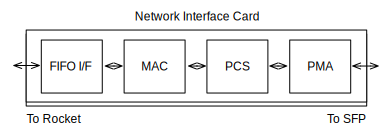
\includegraphics[width=\linewidth]{../../img/NIC.pdf}
\caption{ZC706-Compatible NIC from Xilinx IP}
\end{center}
\end{figure}

    Our system uses Xilinx IP included in Vivado $2014.2$ in order to construct 
    a 1Gbps Network Interface Card. The first of these components is the LogiCORE
    IP Ethernet 1000Base-X PCS/PMA or SGMII core \cite{pcspma}. The PCS/PMA
    core implements the 1000Base-X Physical Coding Sublayer and Physical Medium
    Attachment standards, as described in IEEE 802.3-2008. The core integrates
    a device specific transceiver that is compatible with our Brocade SFP Module.
    On the client side, the PCS/PMA core provides an MDIO interface for control
    and a GMII interface for data.

    The second component of the NIC is the Xilinx LogiCORE IP Tri-Mode Ethernet 
    MAC \cite{trimac}. The MAC implements the Ethernet Medium Access Controller
    protocol as defined in the IEEE 802.3-2008 specification. The MAC handles
    ethernet framing protocols and error detection. It attaches to the PCS/PMA
    IP through a GMII interface for data and an MDIO interface for control.
    On the CPU-side, the core exposes AXI4-Stream interfaces for transmit and 
    receive and an AXI4-Lite Interface for management \cite{axi}. Both of these
    interfaces attach to custom hardware interfaces added to the Rocket core.


\subsection{Bootstrapping the System}
    \subsubsection{ARM Core}

    When power is first supplied to the board, our full-system design, containing
    Rocket along with the traffic manager, accelerator, DMA engine, and NIC is 
    pushed onto the programmable logic in the Zynq SoC. Next, a copy of Linux
    with support for SFP clock bringup is booted on the ARM cores in the Zynq
    SoC. The \texttt{fesvr-zynq} application then executes on the ARM core. 
    This program copies a specified RISC-V binary into the Rocket Core's DRAM 
    over the HTIF bus and resets the Rocket Core. In our case, we supply a 
    \texttt{vmlinux} binary containing the RISC-V Linux kernel, along with a 
    root filesystem.

    \subsubsection{Rocket Core}

    From this point forward, the Rocket Core executes independently of the ARM 
    core. The ARM core now handles only non-network I/O for the Rocket core over
    the HTIF bus. Upon boot, the Rocket core uses our custom TEMAC driver to 
    bring up the NIC, using custom control registers for configuration of the
    NIC and DMA engine.


\subsection{Future Infrastructure Work}
    Although our system functions correctly, we do not adhere to the RISC-V
    I/O specifications. (TODO: maybe this section is unnecessary)

    The resource utilization of our full system is noted in Figure \ref{fig:utiltab}.
    

\begin{figure}[t]
\begin{center}
\label{fig:utiltab}
\begin{tabular}{ | c | c | c |  } \hline
    Resource        & w/o A+TM & w/A+TM  \\ \hline
    Slice LUTs      & 17.09\%   &  21.79\%   \\  \hline
    Slice Registers & 6.18\%    &  8.01\%    \\  \hline
    Memory          & 21.65\%   &  63.85\%   \\  \hline
\end{tabular}
\caption{ZC706 System Utilization}
\end{center}
\end{figure}




\end{frame}

\begin{frame}{Developing a NIC for RISC-V}
    \begin{itemize}
\item Built first RISC-V hardware device: register-mapped NIC
	\begin{itemize}
	\footnotesize
	\item Programmed I/O with custom Linux kernel driver
	\item First \texttt{telnet/ssh} session into a physical RISC-V machine
	\end{itemize}
\end{itemize}
\begin{center}
        \includegraphics[scale=0.3]{../img/first_telnet.png}
    \end{center}

\begin{itemize}
\item Evolved to DMA-based NIC for performance
\end{itemize}
\end{frame}



\begin{frame}{Raw Latency Comparison}
    \includegraphics[width=\linewidth]{../img/graph.png}
\end{frame}


\begin{frame}{Facebook ETC Benchmark}
    \includegraphics[width=\linewidth]{../img/facebook_etc_for_pres.png}
\end{frame}





\begin{frame}{Demo}
\begin{multicols}{2}
\centering
\alert{Baseline} \\[0.5\baselineskip]
\includegraphics[scale=0.5]{../img/system-base.pdf}

\columnbreak

\centering
\alert{Enhanced} \\[0.5\baselineskip]
\includegraphics[scale=0.5]{../img/system-kvstore.pdf}
\end{multicols}
\end{frame}


\begin{frame}{Conclusion/Future Work}
    \begin{itemize}
        \item We added networking support to the Rocket Core and built a key-value store accelerator that reduces get-request latency
            \begin{itemize}
                \item Raw performance: achieved 10x reduction in latency
                \item Able to serve 40\% of keys in a realistic workload at this reduced latency
            \end{itemize}
        \item Based on ZC706 Utilization, lots of room to expand/explore
        \item Future integration between Jackhammer, Xilinx Vivado, and Benchmarking Scripts for FPGA DSE
        \item Investigate replacing fixed-function traffic manager with programmable co-processor 
    \end{itemize}


\begin{center}
    ZC706 (FPGA) Utilization

\vspace{3mm}
\begin{tabular}{ | c | c | c |  } \hline
    Resource        & w/o A+TM & w/A+TM  \\ \hline
    Slice LUTs      & 17.09\%   &  21.79\%   \\  \hline
    Slice Registers & 6.18\%    &  8.01\%    \\  \hline
    Memory          & 21.65\%   &  63.85\%   \\  \hline
\end{tabular}
\end{center}
\end{frame}



\begin{frame}{Questions?}
\end{frame}

\end{document}
